\subsubsection{Almeida-Pineda Algorithm}

Pineda first applied the backpropagation rule to recurrent networks. Recurrent networks can have cycles and they contain no layers. Subset $\Omega$ of the units is treated as the output layer. So the Almeida-Pineda network is a generealization of the backpropagation network. 

As the network is recurrent it can remember information and can be used as CAM.
%TODO citation for CAM 

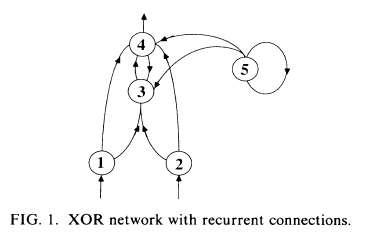
\includegraphics[width=8px]{img/recurrent.png}

\paragraph{My notes.} 
So the Pinedas NS is a dynamical system which should converge and converges for forward/backward nets (quite trivially). 

The delta rule is constructed to move the state towards the fixed point which is defined so that the difference on output neurons is equal to zero (values on other neurons are chosen arbitrary?). 

First Pineda derives an exact learning rule which requires computation of inverse matrix what is both bad for implementation and biological plausibility. So it is simplified to associate dynamical system (I don't understand how) which converges if the original dynamical system converges (proved by Almeida). 

It is more natural as all neurons are equivalent by construction. The advantage is exploited in hardware computation as it treats differential equations more naturally can be solved by analog computers. 

%TODO: Compare this conclusion with O'Reillys. 


TODO: Understand the basics of differential equations to enhance the intuition about learning rules. 

TODO: Study the Lapedes and Farber: master / slave NS. 

\paragraph{Citations from the article.}

Nevertheless it has been applied to recurrent networks by taking advanage of the fact that for every recurrent network there exists an equivalent feedforward network (for a finite time) \cite{pineda1987generalization}.

Hopfield's equations are globally asymptotically stable if $w$ is symmetric and has zeros along the diagonal \cite{pineda1987generalization}.

$$y_r = \beta f_r^,(u_r)\sum_k J_k(L^{-1})_{kr},$$
where 
$$L_{ij} = \alpha \delta_{ij} - \beta f_i^,(u_i)w_{ij},$$
and where $\delta_{ij}$ is the Kronecker $\delta$ symbol and $J_i = t_t - x_i$ if $i \in \Omega$ and $J_i = 0$ otherwise \cite{pineda1987generalization}. 

Then the exact learning rule is 
$$dw_{rs}/dt = \gamma y_r x_s.$$
Rhis exact learning rule needs matrix inversion to calculate the error signals $y_k$. Direct matrix inversions are necessarily nonlocal calculations and therefore this learning algorithm is not suitable for implementation as a neural network \cite{pineda1987generalization}. 

TODO: Understand the associated dynamical system and the new learning rule (page 3/4). 

\paragraph{O'Reillys conclusion}
\cite{o1996bio}
The activation states in AP are updated according to a discrete-time approximation of the following dif-
ferential equation, which is integrated over time with respect to the net input terms :

$$\frac{d\eta_j}{d_t} = -\eta_j + \sum w_{ij} \sigma(\eta_i).$$

This equation can be iteratively applied until the network settles into a stable equilibrium state (i.e., until the
change in activation state goes below a small threshold value), which it will provably do if the weights are
symmetric (Hopfield, 1984), and often even if they are not (Galland \& Hinton, 1991).

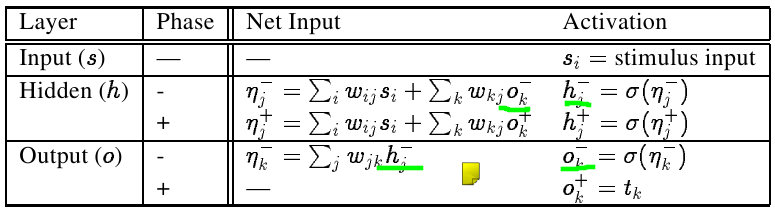
\includegraphics[width=10cm]{img/table_ap.png}
